%\chapter{Principais trabalhos e \emph{datasets} estudados}

%\section{Bitterlemons}
%\label{bitter}

%Falar de tudo e dos pre-processamentos

\chapter{Classificação por perspectiva: revisão e discussão}
\label{chap3}

A classificação de documentos de acordo com suas perspectivas é um tópico de pesquisa relativamente novo. Ele foi proposto como subproblema da área de Mineração de Opinião em 2008, pelas pesquisadoras Bo Pang e Lillian Lee \cite{omsa}. De acordo com elas, esse subproblema se diferencia da classificação por opinião por não configurar as classes como pólos (\emph{positivo}, \emph{negativo} etc.). De fato, a classificação por perspectiva visa a separar os documentos de um corpus de acordo com pontos de vista diferentes, como \emph{pró-Israel} ou \emph{pró-Palestina}. Embora, em certo nível, isso também polarize o corpus, já que normalmente os pontos de vista são antagônicos, dividi-lo de acordo com suas perspectivas é uma tarefa mais subjetiva do que aquela envolvendo opiniões. Um bom exemplo da diferença entre um ponto de vista e uma opinião, no contexto dos trabalhos revisados e de acordo com a \emph{survey} de Pang e Lee, é o seguinte: \emph{'Matrix' é um filme excelente} (opinião sobre um objeto específico, mais pontual) e \emph{a paz mundial dificilmente será alcançada} (ponto de vista sobre um tema; algo que pode implicar em uma série de opiniões alinhadas com este pensamento). Apesar de ter sido proposto formalmente apenas em 2008, uma conferência importante para a área de Mineração de Opinião, a \emph{AAAI\footnote{\emph{Association for the Advancement of Artificial Intelligence}.} Conference}, lançou, na edição de 2010, uma trilha específica para trabalhos nesta direção: \emph{Sentiment and Perspective} \cite{aaai2010}. Isso indica que o subproblema deve se fortalecer como área de pesquisa nos próximos anos.

A \emph{survey} de Pang e Lee, uma das principais referências para este projeto, elenca três trabalhos que fazem classificação por perspectiva, publicados entre os anos de 2004 e 2006. Assim como nesse \emph{survey}, esta monografia enfoca trabalhos recentes, publicados entre 2000 e 2010. A metodologia aplicada na busca por trabalhos a serem revisados pode ser resumida nos seguintes passos:

\begin{enumerate}
\item Consideração dos três trabalhos indicados na \emph{survey} de Pang e Lee;
\item Busca, no \emph{Google Scholar}, por trabalhos citados nesses artigos;
\item Busca, no \emph{Google Scholar}, por trabalhos que citam os artigos coletados nos itens anteriores;
\item Busca, na \emph{ACL Anthology}\footnote{A \emph{Association of Computational Linguistics}, \emph{ACL}, mantém o maior arquivo digital envolvendo trabalhos de Linguística Computacional, o que inclui Mineração de Opinião (http://aclweb.org/anthology-new/).} pelas palavras \emph{perspective}, \emph{viewpoint}, \emph{politics}, \emph{political}, \emph{ideology} e \emph{ideological}. Estas palavras foram escolhidas por (1) funcionarem como sinônimos nos artigos coletados anteriormente ou (2) pela relevância em suas temáticas, escritos por especialistas;
\item Busca nos \emph{sites} dos eventos \emph{EMNLP\footnote{\emph{Empirical Methods in Natural Language Processing Conference.}}, NAACL\footnote{\emph{North American Chapter of the Association for Computational Linguistics Conference.}}, AAAI\footnote{\emph{Association for the Advancement of Artificial Intelligence Conference.}}} e \emph{CoNNL\footnote{\emph{Computational Natural Language Learning Conference.}}}, realizados entre 2000 e 2010, pelas mesmas palavras do item anterior. Esses eventos foram selecionados pela relevância na área de Mineração de Opinião. 
\end{enumerate}

Nem todos os trabalhos coletados, de acordo com essa metodologia, tinham necessariamente a ver com classificação por perspectiva. Alguns, como a tese de Alice Oh, se propõem modelar computacionalmente o conceito de perspectiva \cite{alice-oh}; outros, como o artigo de Laver et al., se propõem a criar uma escala ideológica e comparar documentos de acordo com ela \cite{wordscores}.  Por este motivo, foi feita uma filtragem que resultou em 14 trabalhos a serem revisados. Na seção \ref{freqs:revisao}, essa revisão é apresentada. Quase todos os trabalhos consideram, ainda que não exclusivamente, as contagens de palavras dos documentos na classificação. Além disso, eles divergem bastante quanto à escolha de outras características dos documentos. Por estes motivos, a seção \ref{freqs:experim} discute a relação entre a classificação baseada em contagens de palavras e o emprego delas por diferentes perspectivas. Por fim, na seção \ref{freqs:conc}, apresentam-se conclusões sobre os conteúdos expostos nas seções \ref{freqs:revisao} e \ref{freqs:experim}. 

\section{Trabalhos Revisados}
\label{freqs:revisao}

Todos os trabalhos revisados nesta seção apresentam uma metodologia em comum: eles organizam um corpus de documentos, definem em que perspectivas ele se divide, eventualmente pré-processam os documentos e, em seguida, classificam-nos utilizando alguma técnica - na maioria dos casos, SVMs ou Naïve Bayes. Independentemente da forma de classificação, tem-se que elas sempre se baseiam em características dos documentos para determinar suas classes. 
Quase todos os trabalhos revisados nessa seção exploram, como características, (1) contagens de palavras, ausência/presença de palavras ou alguma variação delas. Boa parte deles não testa o uso de nenhuma outra característica; alguns trabalhos as comparam com outras, que normalmente são seu enfoque. Essas outras características são escolhidas de forma muito particular, variando de um trabalho para outro. Em vez de apenas considerarem ocorrências de palavras em textos, esses trabalhos exploram (2) suas relações sintáticas, suas semânticas e também valores associados à proximidade temática/semântica entre dois ou mais documentos. Dado que essas últimas características variam bastante, e considerando também a popularidade das primeiras, decidiu-se dividir a revisão dos trabalhos nas seguintes subseções: a subseção \ref{contagem} apresenta trabalhos que classificam documentos baseando-se exclusivamente em (1); a subseção \ref{sintaxe} apresenta trabalhos que exploram (2) na classificação, exclusivamente ou em conjunto com (1). É importante informar que alguns trabalhos da segunda subseção, por questões comparativas, também classificam documentos exclusivamente de acordo com (1) - mas este não é o foco deles.  Por fim, na subseção \ref{compara}, é apresentada uma pequena análise comparativa envolvendo os trabalhos revisados nas subseções anteriores.

\subsection{Trabalhos que exploram contagem/presença de palavras ou variações}
\label{contagem}

O trabalho de \textbf{Lin et al.} classifica artigos do \emph{site} Bitterlemons\footnote{http://bitterlemons.org/} como pró-Palestina ou pró-Israel \cite{lin-et-al2006}. Inicialmente, os documentos são representados como listas de palavras reduzidas a seus radicais. Isso significa, por exemplo, que as palavras \emph{political} e \emph{politics} são representadas através de um mesmo termo, o radical \emph{politic}. Os classificadores Naïve Bayes e SVM são então aplicados, explorando as contagens desses radicais em cada documento. A taxa de acerto obtida com o SVM variou entre 81.48\% e 97.24\%; com o Naïve Bayes, ela variou entre 84.85\% e 99.09\%. Essas variações advêm de diferentes divisões entre os conjuntos de treinamento e teste. Por fim, o trabalho de Lin et al. propõe o classificador \emph{Latent Sentence Perspective Model}, ou simplesmente LSPM. Ele consiste em uma variação do Naïve Bayes que, em vez de considerar documentos como listas de palavras, os representa como listas de senteças. A hipótese assumida por ele é a seguinte: nem todas as sentenças carregam um ponto de vista, de modo que o classificador, antes de definir a classe de um documento, deve selecionar quais delas carregam palavras relevantes. A taxa de acerto obtida com o LSPM variou entre  86.99\% e 94.93\%, também como consequência de diferentes divisões entre os conjuntos de treinamento e teste. Para essas divisões, as taxas de acerto obtidas com o Naïve Bayes foram de 84.85\% e 93.46\%. O SVM não foi comparado diretamente com o LSPM. Apesar do desempenho superior a do Naïve Bayes, nenhum outro trabalho revisado faz uso desse classificador. 

\textbf{Mullen e Malouf} propõem dois trabalhos que analisam um conjunto de \emph{posts} do fórum de discussão política Politics\footnote{http://politics.com}. No \textbf{primeiro trabalho}, eles tratam cada documento como a união de todos os \emph{posts} de um mesmo usuário \cite{aaai-politics}. Cada documento é representado como uma lista de palavras, e um Naïve Bayes é aplicado considerando suas contagens em cada documento. A taxa de acerto obtida, via validação cruzada de dez dobras, foi de 60.37\%. O tamanho do \emph{dataset} (apenas 185 documentos) e o uso parecido de palavras por ambas as ideologias foram apontados como alguns dos principais motivos para a obtenção desse resultado. Mullen e Malouf também sugerem que a presença de documentos menores, correspondentes a usuários do fórum que raramente postam, pode contribuir negativamente para o desempenho do Naïve Bayes. Uma última observação desse trabalho indica o que pode estar acontecendo: usuários liberais citam falas de usuários conservadores em 62.2\% de seus \emph{posts}; analogamente, conservadores citam liberais em 77.5\%  de seus \emph{posts}. A presença das perspectivas liberal e conservadora em um mesmo documento, com uma correspondendo às intenções do usuário e outra sendo citada, pode homogeneizar o uso de palavras no corpus, comprometendo a viabilidade da classificação.

%A ideia é que, como esses usuários participam muito pouco do fórum, as palavras em seus \emph{posts} não são suficientes para se consolidar uma perspectiva, tornando-os mais difíceis de se classificar. Restringindo a classificação a usuários que postaram no fórum pelo menos 20 vezes, a taxa de acerto obtida com o Naïve Bayes foi ligeiramente superior (61.38\%).  Embora o artigo não indique a proporção média entre essas citações e o restante dos documentos, é possível que elas estejam interferindo negativamente no aprendizado das perspectivas. 

%Os documentos devem ser classificados, portanto, como alinhados com uma dessas duas ideologias. , escrito por cidadãos comuns dos Estados Unidos \cite{aaai-politics} \cite{malouf-taking_sides}. Em ambos, apesar de admitirem a diversidade de posicionamentos contidos no fórum, os autores dividem os documentos em apenas duas perspectivas, por uma questão de simplicidade: liberal e conservadora.

Essa forma de interação entre os participantes do fórum é explorada pelo \textbf{segundo trabalho de Mullen e Malouf} \cite{malouf-taking_sides}, com o intuito de melhorar a classificação. Para isto, cria-se um grafo de co-citação em que cada vértice representa um participante e cada citação em uma fala a outra é indicada por uma aresta entre seus autores. Os participantes são agrupados de acordo com seus padrões de citação e, em seguida, as falas de cada grupo obtido são tratadas como um único documento. Aplica-se um Naïve Bayes a esta nova coleção de documentos, também explorando apenas suas contagens de palavras, e os resultados obtidos são propagados para todos os participantes de cada grupo. Essa metodologia atinge resultados significativamente melhores do que aqueles obtidos no trabalho anterior: para participantes com mais de 500 palavras de fala no fórum, a taxa de acerto relatada é de 73\%. É válido salientar que, muito provavelmente, o sucesso dessa técnica é consequência do fato de que usuários alinhados ideologicamente não se citam muito. Se, além de citar seus oponentes, eles também se citassem bastante, os padrões de citação seriam sempre muito parecidos, inviabilizando os agrupamentos adequados no grafo.

O trabalho de \textbf{Durant e Smith} constrói um corpus sobre os posicionamentos do ex-Presidente George W. Bush quanto à Guerra do Iraque \cite{durant-smith}. O objetivo desse trabalho é classificar \emph{posts} de diversos \emph{blogs} políticos de acordo com os pontos de vista pró Guerra do Iraque e anti Guerra do Iraque.  Os classificadores Naïve Bayes e SVM foram aplicados, considerando apenas a presença/ausência de palavras nos documentos. A taxa de acerto obtida com um SVM foi de 75.47\%. Com o Naïve Bayes, ela foi de 78.06\%. Os autores, em seguida, investigam se a seleção de apenas parte das palavras pode melhorar a classificação. Eles aplicam uma técnica denominada \emph{CfsSubsetEval}, disponível na ferramenta WEKA 3.4\footnote{http://www.cs.waikato.ac.nz/ml/weka/}, que busca um subconjunto de palavras que maximize a taxa de acerto obtida. As palavras devem ter alta correlação com as classes escolhidas, mas baixa correlação entre si. Aplicando os classificadores SVM e Naïve Bayes, e considerando apenas os subconjuntos selecionados pela técnica, as taxas de acerto obtidas foram de 87.66\% e 89.77\%, respectivamente. É válido ressaltar que a técnica \emph{CfsSubsetEval} pode trazer uma melhoria de desempenho significativa para \emph{datasets} escritos em qualquer língua.

O trabalho de \textbf{Hirst, Riabinin e Graham} constrói dois \emph{datasets}, um em inglês e outro em francês, que consistem de discursos de congressistas canadenses nas reuniões parlamentares \cite{hirst-et-al}. Além de classificar esses discursos como liberais ou conservadores, esse trabalho investiga se as classes correspondem de fato a ideologias diferentes ou, simplesmente, a expressões de ataque e defesa. Inicialmente, os autores analisam o \ensuremath{36^o} parlamento canadense, período em que um partido liberal estava com a maioria no poder. Excluindo apenas as palavras menos frequentes do corpus, e aplicando um SVM baseado apenas nas contagens de palavras dos documentos, as taxas de acerto obtidas foram de 83.8\% e 75.5\% para os corpora inglês e francês, respectivamente. Em seguida, os autores selecionaram o \ensuremath{39^o} Parlamento, período em que os partidos liberais eram oposição, para verificar o que de fato estava determinando a classificação. Treinando com documentos do \ensuremath{36^o} Parlamento e testando com aqueles do \ensuremath{39^o}, a classificação entre liberal e conservador é insatisfatória: as taxas de acerto foram de 44.9\% e 45.7\% para os corpora inglês e francês respectivamente. Treinando com o \ensuremath{39^o} e testando com o \ensuremath{36^o}, as taxas de acerto foram ainda piores: 36.8\% e 35.2\% para os corpora inglês e francês respectivamente. Diante disso, os autores concluem que que as ideologias liberal e conservadora não são exploradas adequadamente pelos discursos. Se o fossem, e considerando que elas não mudaram significativamente de um parlamento para o outro, estes últimos experimentos apresentariam resultados melhores. Eles indicam que os discursos envolvem muitas expressões de ataque e defesa, que mudam de partido conforme eles se alternam no poder. Por este motivo, os conjuntos de treinamento e teste apresentam padrões de ataque e defesa invertidos, implicando no mau desempenho da classificação. Esse trabalho alerta, portanto, para a definição adequada de que perspectivas estão contidas no corpus. Neste caso, em vez de liberal e conservadora, seria mais adequado utilizar pró-governo e anti-governo, ou situação e oposição. % fixam as palavras que ocorrem menos frequentemente nos corpora foram removidas, e um SVM foi aplicado.

O trabalho de \textbf{Klebanov, Beigman e Diermeier} avalia o desempenho dos classificadores Naïve Bayes e SVM, utilizando para isso características diferentes dos documentos. Para o Naïve Bayes, os autores comparam a escolha entre (1) presença/ausência de palavras e (2) contagens de palavras. Para o SVM, as comparações envolvem a escolha entre (1), (3) suas contagens normalizadas em relação ao documento (frequências) e (4) suas frequências ponderadas em relação aos outros documentos do corpus. É válido ressaltar que todas essas características são apenas variações de contagens de palavras. Os autores selecionaram quatro \emph{datasets} para comparar essas escolhas: o primeiro envolve debates sobre o aborto, dividido entre pró-escolha e pró-vida; o segundo consiste em artigos sobre a pena de morte, dividido entre pró pena de morte e anti pena de morte; o terceiro é composto de artigos sobre o conflito Israel-Palestina, escritos por convidados do \emph{site} Bitterlemons e estudados por Lin et al. \cite{lin-et-al2006}; o quarto também é composto de documentos desse \emph{site}, cada um escrito por um especialista diferente. Esses dois últimos, assim como no trabalho de Lin et al., são divididos entre pró-Palestina e pró-Israel.  No caso do Naïve Bayes, o uso de (1) se mostrou melhor em alguns \emph{datasets} e o de (2), em outros. A maior diferença de desempenho observada está relacionada com o corpus de pena de morte: com (1), a taxa de acerto obtida foi de 88\%; com (2), 93\%. Os autores indicam, diante disso, que essa escolha não é tão relevante para problemas de classificação por perspectiva. Quanto ao SVM, a escolha por (1) se mostrou superior ou equivalente às outras em todos os casos. A maior diferença de desempenho observada também está associada ao corpus de pena de morte: enquanto (1) conduz a uma taxa de acerto de 83\%, (3) resulta em 82\% e (4) em 73\%. Esse trabalho, assim como o de Durant e Smith \cite{durant-smith}, também investiga o uso de um subconjunto de palavras. Com o apoio do \emph{toolkit} WEKA, os autores selecionam subconjuntos pequenos, contendo entre 100 e 500 palavras, e indicam que a classificação dos \emph{datasets}, nestes casos, conserva seu desempenho. As taxas de acerto não aumentam, como no trabalho de Durant e Smith, mas também não diminuem.




%esses dois pontos de vista. Inicialmente, foi feita uma seleção de \emph{blogs} baseada no \emph{site The Moderate Voice}\footnote{http://themoderatevoice.com/}. Este \emph{site} elenca \emph{blogs} de esquerda, direita e moderados. Para esse trabalho, Durant e Smith exploraram apenas os \emph{blogs} de esquerda e direita. Em seguida, apenas os \emph{posts} que tratavam de Bush e da Guerra do Iraque foram separados para classificação. O material foi dividido por mês, devido à grande quantidade de \emph{posts}. Esse trabalho assume que \emph{blogs} de esquerda concentram o ponto de vista anti-Bush,  no que diz respeito a suas atitudes quanto à Guerra do Iraque. \emph{Blogs} de direita, por sua vez, concentram o ponto de vista pró-Bush. 


%O tutorial de Resnik e Hardisty sobre Naïve Bayes e LSPM sugere algumas equações para a implementação deste último \cite{resnik}, mas o próprio Resnik afirmou, em \emph{e-mail} endereçado à autora desta monografia, nunca ter conseguido replicar os resultados apresentados por Lin et al. \cite{email}. Aparentemente, portanto, o LSPM não é tão simples de implementar quanto o Naïve Bayes.  Lin et al. concluem, diante dessas comparações, que o LSPM apresenta desempenho superior ao do Naïve Bayes. N


%Os artigos foram extraídos do \emph{site} Bitterlemons\footnote{http://www.bitterlemons.org/} e estão divididos entre \emph{Palestinian} ou \emph{Israeli}. Os primeiros defendem pontos de vista pró-Palestina; os segundos, pró-Israel. Essa divisão é explorada mais à frente, de modo que o




\subsection{Trabalhos que exploram outras características dos documentos}
\label{sintaxe}

O trabalho de \textbf{Jiang e Argamon} constrói um corpus de documentos extraídos de \emph{blogs} sobre política escritos em inglês \cite{jiang-argamon}. Cada \emph{blog} é associado à perspectiva liberal ou conservadora, divisão explorada na classificação. Os documentos que constituem o corpus são apenas as páginas iniciais de cada um deles. Inicialmente, Jiang e Argamon aplicam um SVM às páginas, considerando apenas a presença/ausência de palavras nos documentos. A taxa de acerto obtida foi de 81.92\% e, considerando ambas as classes, tem-se que a precisão média foi de 81.76\%, a rechamada média foi de 81.93\% e a métrica F1 média foi de 81.79\%. Em seguida, as páginas foram reduzidas a suas sentenças subjetivas, através de uma seleção baseada no dicionário semântico \emph{General Inquirer}\footnote{http://www.wjh.harvard.edu/~inquirer/}. Para uma sentença ser escolhida, ela deveria conter pelo menos duas palavras categorizadas, segundo o dicionário, como pertencentes às categorias \emph{Dor}, \emph{Hostilidade}, \emph{Prazer} ou \emph{Virtude}, dentre outras. A taxa de acerto, neste cenário, subiu para 83.28\%. As precisão, rechamada e métrica F1 médias foram de, respectivamente, 83.26\%, 83.38\% e 83.24\%. Esse trabalho, por fim, busca extrair as expressões opinativas que mais se relacionam aos pontos de vista liberal e conservador, baseando-se nas sentenças subjetivas e em consultas ao dicionário \emph{General Inquirer}. O SVM é aplicado considerando a presença/ausência de palavras e, adicionalmente, a presença/ausência das expressões opinativas separadas para cada lado. A taxa de acerto neste cenário foi de 84.96\%. As precisão, rechamada e métrica F1 médias foram de, respectivamente, 83.24\%, 83.48\% e 83.27\%. As melhorias em relação ao uso exclusivo de ausência/presença de palavras, portanto, são pequenas. Além disso, essas metodologias não são facilmente adaptáveis a línguas que não dispõem de dicionários como o \emph{General Inquirer} \emph{online}.

%Apesar de melhorarem a taxa de acerto obtida inicialmente, essas metodologias são completamente dependentes da língua em que o corpus está escrito. Elas não são  % Os \emph{blogs} foram escolhidos de acordo com cinco catálogos \emph{online}: BlogCatalog, Blogorama, eTalkingHead, Campaigns and Elections e Best of the Web Blogs\footnote{http://blogcatalog.com, http://blogarama.com, http://etalkinghead.com, http://campaignsandelections.com e http://blogs.botw.org.}. A finalidade desse trabalho, portanto, é determinar o posicionamento político desses \emph{blogs}, considerando seu conteúdo mais imediato - suas páginas iniciais. %As metodologias empregadas são completamente dependentes da linguagem do corpus, por utilizarem dicionários desenvolvidos para o inglês. % português.

O trabalho de \textbf{Greene e Resnik} enfoca no estudo de um corpus sobre a pena de morte \cite{greene}. Esse corpus é posteriormente analisado no trabalho de Klebanov, Beigman e Diermeier \cite{klebanov}, apresentado na seção anterior. O objetivo do trabalho é classificá-lo de acordo com as perspectivas pró pena de morte e anti pena de morte, e a metodologia desenvolvida baseia-se na hipótese de que existe uma conexão entre a estrutura de uma sentença e seu ponto de vista. Neste sentido, os autores selecionam um conjunto de verbos relevantes no corpus, como \emph{kill} e \emph{murder}, e criam representações para todos os termos que se relacionam sintaticamente com eles. Essas representações consistem em tuplas que associam cada termo a seu papel sintático na frase. Esses papéis, por sua vez, podem ser \emph{sujeito}, \emph{objeto direto}, \emph{verbo transitivo}, dentre outros. A determinação desses papéis foi feita com o apoio do programa \emph{Stanford Parser}\footnote{http://nlp.stanford.edu/software/lex-parser.shtml}, adaptado à língua inglesa. Greene e Resnik então aplicam um SVM nos documentos reduzidos a essas representações, atingindo taxas de acerto de 82.09\% e 88.10\%, a depender da escolha de verbos. Em vez de uma lista de palavras, portanto, o SVM é aplicado a uma lista de tuplas. Para comparar sua metodologia, os autores aplicam o SVM a documentos representados como sequências de duas palavras (bigramas), todas reduzidas a seus radicais. Nesse caso, as taxas de acerto obtidas foram de 68.37\% e 71.96\%, também a depender da escolha dos verbos. Essa metodologia, portanto, traz uma melhoria muito significativa para a classificação desse corpus. Apesar disso, aplicando a mesma metodologia ao corpus sobre o conflito Israel-Palestina, estudado por Lin et al. \cite{lin-et-al2006}, Greene e Resnik não obtêm nenhuma melhoria significativa. Em alguns cenários, os resultados obtidos por Lin et al. são ligeiramente melhores; em outros, são aqueles apresentados por estes autores.

O trabalho de \textbf{Efron} constrói dois \emph{datasets}: um envolvendo artigos sobre a política dos Estados Unidos e outro composto de textos sobre artistas musicais \cite{efron}. O primeiro corpus é classificado de acordo com as perspectivas direita e esquerda e o segundo, de acordo com as orientações pró-alternativa ou pró-popular. Inicialmente, Efron classifica os dois corpora com um Naïve Bayes e um SVM. O autor não especifica se são utilizadas contagens de palavras ou alguma outra característica, mas afirma que os dois métodos se baseiam apenas nas palavras contidas nos textos. Com o Naïve Bayes, as taxas de acerto obtidas nestes corpora foram de, respectivamente, 64.71\% e 50.1\%. Para o primeiro corpus, a taxa de acerto obtida com um SVM foi de 72.96\%; quanto ao segundo, não foram realizados experimentos com o SVM por carência de recursos computacionais. A fim de melhorar as taxas de acerto,  Efron desenvolve uma classificação baseada em citações que não envolve contagens de palavras nem citações de um documento a outro, mas sim suas semelhanças temáticas. Na prática, Efron determina a perspectiva de cada documento de acordo com a probabilidade deles serem co-citados com  documentos fixados como referência para cada perspectiva. Essa probabilidade é estimada a partir dos números de documentos retornados pelo buscador AltaVista\footnote{http://altavista.com/} quando dois documentos são buscados, indicando co-citação entre eles. Essa metodologia de classificação, aplicada ao primeiro \emph{dataset}, resultou em uma taxa de acerto de 94.1\%. Quanto ao segundo, as taxas de acerto obtidas foram de 82.18\% e 88.84\%. No primeiro caso, todos os documentos foram considerados; no segundo, os menos co-citados foram descartados. Apesar de simples e aparentemente eficiente, essa metodologia apresenta uma séria limitação: se o corpus for composto de documentos pouco citados na Web, as classes podem ser estimadas erroneamente com uma alta frequência, não trazendo nenhuma melhoria significativa à classificação.

O trabalho de \textbf{Thomas, Pang e Lee} se propõe a determinar os pontos de vista de congressistas dos Estados Unidos quanto a novas leis \cite{get-out-the-vote}. O corpus é dividido entre as perspectivas suporte e oposição em relação a novas leis, e cada documento corresponde, a princípio, a uma fala de um congressista. Inicialmente, cada texto é classificado de forma isolada, através da aplicação de um SVM que considera a presença/ausência de palavras em cada um deles. As taxas de acerto obtidas foram de 66.05\% e 70.04\%, a depender do subconjunto de documentos classificado. Tratando cada documento como a concatenação de todas as falas de um mesmo congressista, as taxas obtidas com o SVM, considerando as mesmas características, foram de 70.00\% e 71.60\%. A fim de melhorar essas taxas de acerto, os autores comparam trechos de documentos e determinam valores positivos que representam o quanto eles concordam. Quando esses valores são menores do que um determinado \ensuremath{\theta} fixado, considera-se que não há indícios suficientes de que os documentos concordam; eles são, então, reduzidos a zero. Adicionalmente, os autores aproveitam os experimentos com o SVM para determinar o grau de preferência para classificar cada documento como suporte ou oposição. A classe escolhida para cada um deles deve ser aquela que favorece o seguinte cenário: (1) ela não deve, idealmente, ser a rejeitada pelo SVM e (2) documentos que concordam muito não devem ser associados a classes diferentes. As taxas de acerto obtidas, considerando cada documento como uma fala, variaram entre 70.81\% e 89.11\%, a depender do subconjunto classificado e do valor de \ensuremath{\theta}. Considerando cada documento como a concatenação de todas as falas de um mesmo congressista, as taxas de acerto obtidas variaram entre 71.28\% e 88.72\%, também a depender do subconjunto classificado e do valor de \ensuremath{\theta}. A determinação errônea de concordâncias entre documentos pode prejudicar significativamente a classificação. Além disso, de acordo com os próprios autores, a adoção dessa metodologia só traz benefícios quando há artigos difíceis de classificar individualmente.    

O trabalho de \textbf{Bansal, Cardie e Lee} propõe uma extensão ao trabalho de Thomas, Pang e Lee \cite{get-out-the-vote}, considerando também a \emph{discordância} entre documentos \cite{disagree}. A hipótese assumida em ambos os trabalhos é a mesma: se é difícil determinar a classe de um documento \emph{x}, mas sabe-se que ele concorda \emph{ou discorda} de um documento \emph{y}, fácil de classificar, a determinação da classe de \emph{x} também se torna mais fácil. O trabalho apresenta algumas estratégias para determinação dos valores de discordância e, em seguida, compara seus usos com a metodologia proposta por Thomas, Pang e Lee. Bansal, Cardie e Lee também lidam com valores negativos, associados à discordância. Na prática, é preciso mapear esses valores negativos em positivos, pois eles dificultam o problema de otimização envolvido na determinação das classes dos documentos. Esses mapeamentos são justamente o que diferencia uma estratégia de outra. Utilizando o mesmo \emph{dataset} analisado por Thomas, Pang e Lee, os autores deste trabalho obtêm resultados superiores ou equivalentes àqueles que consideram apenas a concordância entre documentos, para a maioria das estratégias testadas. As taxas de acerto, entretanto, não são informadas explicitamente neste trabalho, sendo representadas através de um gráfico comparativo.
%convote e disagree
%decidem considerar o quanto congressistas diferentes \emph{concordam}. Neste sentido, os autores 



\subsection{Comparações}
\label{compara}

Os trabalhos revisados nesta seção propõem, em quase todos os casos, \emph{datasets} relacionados com questões políticas. Neste sentido, o trabalho de \textbf{Efron}, revisado na subseção \ref{sintaxe}, destaca-se por também abordar perspectivas sobre música (pró-alternativa e pró-popular) \cite{efron}. De fato, não é simples definir o que é um ponto de vista ou perspectiva, mas, considerando-se a discussão proposta na \emph{survey} de Pang e Lee \cite{omsa}, essas terminologias não abrangem apenas temáticas políticas - mesmo que seja mais fácil visualizá-las nesses contextos. Adicionalmente, Alice Oh, em seu trabalho sobre modelagem de perspectiva, aborda uma temática esportiva (jogos de \emph{baseball}) \cite{alice-oh}. Embora ela não lide com classificação, seu estudo envolve as perspectivas sobre os jogos, evidenciando que é possível explorar temáticas não-políticas. Seria interessante, portanto, ampliar os estudos de classificação por perspectiva para outros domínios sócio-culturais. Por fim, é importante escolher essas perspectivas com certo cuidado, de modo que elas correspondam efetivamente ao conteúdo do corpus. Neste sentido, o trabalho de \textbf{Hirst, Riabinin e Graham}, apresentado na subseção \ref{contagem}, apresenta uma boa discussão \cite{hirst-et-al}. 

Quanto à definição de perspectivas, todos os trabalhos revisados dividiram seus corpora em duas delas, associando cada uma a uma classe. Embora essas divisões sejam mais complexas do que o uso de pólos positivo e negativo, muito comum na classificação por opinião \cite{thumbs-up} \cite{peanut-gallery}, eles também contêm um  antagonismo, como no caso de \emph{liberal} e \emph{conservador}. Grande parte dos corpora estudados não foi pré-processada. Neste sentido, destaca-se o segundo trabalho de \textbf{Mullen e Malouf}, apresentado na subseção \ref{contagem} \cite{malouf-taking_sides}. Apesar da classificação em si ser simples, baseando-se apenas em contagens de palavras, a geração dos documentos envolve a formulação de um grafo e a análise de padrões de citação semelhantes. Esse foi o pré-processamento mais sofisticado, dentre os trabalhos revisados. No que diz respeito aos classificadores, foi observado que não há consenso quanto à escolha pelo Naïve Bayes ou por um SVM, principais técnicas abordadas. Aparentemente, o desempenho de ambos não difere muito; o que realmente apresenta um impacto na classificação é a escolha das características dos documentos, exploradas por algum dos classificadores. De todo modo, \textbf{Lin et al.} enfoca, em seu trabalho revisado na subseção \ref{contagem}, no desenvolvimento de um novo classificador, o LSPM \cite{lin-et-al2006}. Esse classificador apresenta um desempenho apenas um pouco superior ao do Naïve Bayes, além de não ter sido explorado por nenhum outro trabalho pesquisado. Por outro lado, os trabalhos de Efron, \textbf{Thomas, Pang e Lee} e \textbf{Bansal, Cardie e Lee} apresentam metodologias de classificação completamente diferentes do Naïve Bayes e dos SVMs, e obtêm melhorias significativas em seus resultados \cite{efron} \cite{get-out-the-vote} \cite{disagree}. Essas metodologias, entretanto, se fundamentam na exploração de um tipo de característica: a semelhança entre documentos. Elas não são genéricas como os SVMs, por exemplo. 

Os trabalhos revisados exploram características diferentes dos documentos e, até quando exploram as mesmas, podem escolher apenas um subconjunto delas ou investir no pré-processa mento dos documentos. Tudo isso contribui para a riqueza metodológica desses trabalhos, de modo que ainda não há consenso sobre qual é a melhor forma de classificar documentos de acordo com suas perspectivas. Aparentemente, a resposta para essa questão depende do cenário. Em alguns casos, a simples aplicação de um Naïve Bayes ou um SVM, baseando-se em contagens de palavras, já conduz a bons resultados. É o caso dos trabalhos de Lin et al., Hirst, Riabinin e Graham e \textbf{Klebanov, Beigman e Diermeier}, revisados na subseção \ref{contagem}, e de \textbf{Jiang e Argamon}, revisado na subseção \ref{sintaxe} \cite{lin-et-al2006} \cite{hirst-et-al} \cite{klebanov} \cite{jiang-argamon}. Em outros casos, é possível melhorar o desempenho utilizando \emph{ainda} apenas contagens de palavras. Nestes casos, a estratégia envolve mudar o pré-processamento dos documentos, como no segundo trabalho de Mullen e Malouf, ou escolher um subconjunto ótimo de palavras, como no trabalho de \textbf{Durant e Smith} \cite{malouf-taking_sides} \cite{durant-smith}. Quando essas mudanças não são suficientes, sugere-se a investigação do uso de outras características, como indicam os trabalhos de \textbf{Greene e Resnik}, Efron e Thomas, Pang e Lee, revisados na subseção \ref{sintaxe} \cite{greene} \cite{efron} \cite{get-out-the-vote}. O uso de outras características normalmente envolve a aplicação de \emph{softwares} de apoio e outros algoritmos, de modo que é melhor verificar antes se um Naïve Bayes ou SVM, baseado na simples contagem de palavras, já não resolve o problema. Além disso, a exploração de outras características nem sempre é facilmente adaptável a qualquer língua, como evidenciam os trabalhos de Greene e Resnik e Jiang e Argamon, e nem sempre apresentam uma melhoria significativa em relação a metodologias mais simples, como nesse último caso \cite{greene} \cite{jiang-argamon}.
 
\section{Experimentos com L-LDA e Naïve Bayes}
\label{freqs:experim}

Se um classificador utiliza apenas as contagens de palavras dos documentos para identificar suas perspectivas, sua taxa de acerto é tão mais baixa quanto menos essas contagens mudam de uma perspectiva para outra. Apesar dessa relação ser evidente, não se conhece nenhum método para quantificá-la. Como o seu entendimento amplia a compreensão dos resultados obtidos com esses classificadores, esta seção se detém a ilustrá-la através de alguns experimentos. A ideia é comparar a forma como as palavras são usadas em dois \emph{datasets}: no primeiro, a taxa de acerto obtida com um classificador \textbf{Naïve Bayes}, considerando apenas contagens de palavras, deve ser alta; no segundo, baixa. Para a análise do uso das palavras, será utilizado o modelo de tópicos \textbf{L-LDA}. A escolha do Naïve Bayes advém do fato de que os \emph{datasets} explorados nesta seção não são muito grandes, e o desempenho desse classificador, nesses casos, tende a ser superior ao obtido com SVMs \cite{ng-jordan}. O uso do LSPM não foi cogitado, devido aos pontos discutidos na seção \ref{sec:aaai}.

%APRESENTE OS DOIS DATASETS. JUSTIFIQUE PQ REFEZ EXPERIMENTOS OU PQ N ESCOLHEU O AAAI E SIM OUTRO. - OK 

O primeiro \emph{dataset} estudado é o mesmo discutido na seção \ref{sec:lin-et-al}, composto de artigos sobre o conflito Israel-Palestina. A taxa de acerto obtida com um Naïve Bayes aplicado a esse corpus foi alta, variando entre 84.85\% a 93.46\%. Inicialmente, pensou-se em estudar também o corpus discutido na seção \ref{sec:aaai}, composto de \emph{posts} do fórum Politics.com. O Naïve Bayes não classificou muito bem seus documentos,  atingindo taxas de acerto entre 60.37\% e 64.48\%. Infelizmente, não foi possível obtê-lo mediante solicitação aos autores do artigo. Por este motivo, o segundo \emph{dataset} estudado provém de outro trabalho: o artigo de Thomas, Pang e Lee sobre classificação de perspectiva em debates políticos dos Estados Unidos \cite{get-out-the-vote}. Esse trabalho, cujo corpus está disponível na página de Lee\footnote{http://www.cs.cornell.edu/home/llee/data/convote.html}, é um dos três que não utilizam apenas contagens de palavras para a classificação, sendo detalhado no Capítulo \ref{outros}. Por ora, é suficiente informar que ele é composto de \textbf{8126} trechos de discursos em debates da \emph{House of Representatives}, um dos dois órgãos principais do poder legislativo federal dos Estados Unidos. Os documentos estão divididos de acordo com duas orientações políticas antagônicas: a republicana  (4044) e a democrata (4046). Como no artigo original outras propriedades dos documentos foram consideradas, foi necessário aplicar o Naïve Bayes a esses documentos, considerando apenas as contagens de palavras dos mesmos. No trabalho de Thomas, Pang e Lee, os resultados apresentados são bons - no experimento efetuado com o Naïve Bayes para esse capítulo, entretanto, a taxa de acerto obtida, via validação cruzada de dez dobras, foi de 54.01\%\footnote{A precisão obtida foi de 54.47\% e a métrica F1 foi de 51.42\%.}.  

%MOSTRE COMO OS MODELOS DE TÓPICOS SÃO USADOS NOS DOIS LADOS - ok

Em ambos os \emph{datasets}, cada documento foi associado a dois tópicos: um genérico, idêntico para todos eles, e outro referente à sua perspectiva. No primeiro corpus, essas perspectivas são pró-Israel ou pró-Palestina; no segundo, republicana ou democrata. Há portanto, em cada corpus, três tópicos diferentes. O uso de um tópico genérico associado a todos os documentos ajuda a identificar palavras muito comuns nos \emph{datasets}, independentemente de perspectiva. Essa é a diferença fundamental entre essa aplicação do L-LDA\footnote{A implementação de L-LDA utilizada está disponível no repositório online de Alexandre Passos (http://github.com/alextp).} e a simples contagem de palavras em documentos, dividida entre duas perspectivas. Esse tipo de contagem não evidencia que palavras são mais escolhidas em documentos escritos sob uma certa perspectiva e quais são muito utilizadas por todos eles - informação que colabora para um maior entendimento das taxas de acerto supracitadas, obtidas com um Naïve Bayes. 

%MOSTRE AS PALAVRAS ELENCADAS E DISCUTA

As dez palavras mais frequentemente associadas a cada tópico, retirando-se artigos, conjunções, preposições, advérbios e pronomes pessoais, estão listadas nas Tabelas 4.1 e \ref{freqs:tab2}. Apesar de pequenas, essas listagens sugerem interpretações sobre como as palavras de cada corpus são exploradas por suas diferentes perspectivas. Essas interpretações, essencialmente  subjetivas, ajudam a entender o comportamento do classificador Naïve Bayes aplicado aos dois \emph{datasets}.%colaboram parsubjetiva de se ampliar a discussão sobre os resultados obtidos com o Naïve Bayes.

%provêem informações subjetivas sobre a linguagem empregada nos corpora.
%As palavras extraídas a partir da aplicação de um L-LDA  Ainda assim, essas informações 

%Para ilustrar a relação que existe entre as taxas de acerto do Naïve Bayes e o uso de palavras nesses corpora, a

%As análises feitas a partir dessas pequenas listagens são essencialmente subjetivas, sugerindo interpretações %sugerindo  Essa análise não pretende  % A partir disso, espera-se compreender melhor o 

\begin{table}[h]
\label{tab1}
\centering
\begin{tabular}{| l | p{10cm} | }
\hline
\textbf{Tópico} & \textbf{Palavras} \\ \hline
\textbf{Genérico} & israel, palestinian, israeli, palestinians, state, one, two, israelis, political, right \\ \hline
\textbf{Pró-Israel} & sharon, palestinian, arafat, peace, israeli, prime, bush, minister, american, process \\ \hline
\textbf{Pró-Palestina} & palestinian, israeli, sharon, peace, occupation, international, political, united, people, violence \\ \hline
\end{tabular}
\caption{As dez palavras mais frequentemente associadas aos tópicos pró-Israel, pró-Palestina e genérico, de acordo com um L-LDA.}
\end{table}


Considerando o primeiro corpus, as palavras associadas às perspectivas pró-Israel e pró-Palestina remetem de imediato ao conflito travado entre essas duas nações. Parte delas, como \emph{palestinian} e \emph{israeli}, são bastante mencionadas em ambas as perspectivas, ainda que com propósitos diferentes: %israelenses, 

\begin{quote}

\emph{"The recent \textbf{Israeli} government decision to begin building extensive walls
around \textbf{Palestinian} is just one more example of how \textbf{Israeli} Prime
Minister Ariel Sharon is unable to deal with \textbf{Israeli} problems save
through his narrow security vision."}

{\small Retirado de "Peace in peaces", de Ghassan Khatib (pró-Palestina) - 10/06/2002}
\end{quote}

\begin{quote}

\emph{"The first conclusion that the Israeli political and security
establishment should learn and internalize after 18 months of
\textbf{Palestinian} Intifada, concerns the intensity of \textbf{Palestinian} blind
terrorism and guerilla warfare against the State of Israel."}

{\small Retirado de "The lessons Israel should learn", de Meir Pa'il (pró-Israel) - 29/04/2002}
\end{quote}

%\emph{"Meanwhile, the Israeli army was still suffering in South Lebanon as a result of the dilemma that \textbf{Sharon} put them in."}

%{\small Retirado de "Sharon settles accounts", de Mamdouh Nofal (pró-Palestina) - 28/01/2002}

Outras palavras, como \emph{bush} e \emph{occupation}, foram mais enfatizadas, respectivamente, pelas perspectivas pró-Israel e pró-Palestina, constando em apenas uma listagem. Os trechos abaixo evidenciam a importância, no período em que os documentos desse corpus foram escritos (2001 - 2005), do Governo Bush para Israel e da criação de um Estado para a nação palestina:
 %\textbf{Falar das figuras e de como elas deixam isso tão claro.} 

%\textbf{FIGURAS} % Para compreender melhor o uso das palavras pelos diferentes pontos de vista do corpus, elas foram processadas pelo software wordle22 , resultando nas figuras 7.1, 7.2 e 7.3. O tamanho das palavras nas imagens corresponde ao quanto elas se associam a cada tópico23 .

%Falar das ênfases no próprio lado/lado oposto e mostrar tb as palavras genéricas.
%Os trechos abaixo, separados por perspectiva, ilustram dois contextos diferentes para o uso dessas palavras

%\begin{quote}
%\emph{"The recent \textbf{Israeli} government decision to begin building extensive walls
%around \textbf{Palestinian} is just one more example of how \textbf{Israeli} Prime
%Minister Ariel Sharon is unable to deal with \textbf{Israeli} problems save
%through his narrow security vision."} 

%{\small Retirado de \emph{"Peace in pieces"}, de Ghassan Khatib - 10/06/2002}
%\end{quote}

%\begin{quote}
%\emph{"The first conclusion that the Israeli political and security
%establishment should learn and internalize after 18 months of
%\textbf{Palestinian} Intifada, concerns the intensity of \textbf{Palestinian} blind
%terrorism and guerilla warfare against the State of Israel."} 

%{\small Retirado de }

%\end{quote}


\begin{quote}
\emph{"\textbf{Bush} and his advisers, who have been critical of Clinton's deep involvement
in a failed peace process ever since taking office, nevertheless
understood at the time that peace in the Middle East should be beyond
politics in America, and that the US could not permit itself to turn its
back on an Israeli leader who was determined to make peace."} 

{\small Retirado de "Barak was willing, and so were US Jews", de Yossi Alpher (pró-Israel) - 15/07/2002}
\end{quote}

\begin{quote}
\emph{"But just as we were close to a complete
package that would have ended the \textbf{occupation} and established a
Palestinian state, Barak permitted Ariel Sharon's provocative visit to
Al Aqsa mosque, and launched his "revenge" on Palestinians."} 

{\small Retirado de "Guarding our legitimacy", de Samir Abdullah (pró-Palestina) - 14/10/2002}
\end{quote}

Associadas ao tópico genérico, também estão as palavras \emph{palestinian} e \emph{israeli}, bastante exploradas pelas duas perspectivas. Isso reflete a importância que esses termos têm para o corpus como um todo. Palavras relacionadas mais genericamente ao conflito Israel-Palestina, como \emph{state} e \emph{political}, também aparecem na listagem. %, evidenciando indica que essas palavras         


                     % A imagem 7.3 dá certo destaque a Lula e José Serra, mas também enfatiza outros termos, como governo e brasil, relacionados mais genericamente ao tema geral dos artigos: a política brasileira.


%Essas análises, avaliadas à luz das altas taxas de acerto obtidas com o Naïve Bayes, sugerem que os autores desse primeiro corpus defendem seus pontos de vista veementemente. Como eles são antagônicos, isso se reflete em enfoques diferentes a determinados termos, %empregos diferentes de palavras. % tornando a forma como empregam as palavras  defendem suas perspectivas utilizando palavras de forma suficientemente diferentedestacando ideias diferentes.

\begin{table}[h]
\label{freqs:tab2}
\centering
\begin{tabular}{| l | p{10cm} | }
\hline
\textbf{Tópico} & \textbf{Palavras} \\ \hline
\textbf{Genérico} & mr., speaker, bill, all, time, people, today, gentleman, federal, support \\ \hline
\textbf{Democrata} & bill, security, legislation, states, chairman, country, act, billion, million, law \\ \hline
\textbf{Republicano} & act, chairman, security, states, bill, legislation, 11, support, 9, system \\ \hline
\end{tabular}
\caption{As dez palavras mais frequentemente associadas aos tópicos republicano, democrata e genérico, de acordo com um L-LDA.}
\end{table}

%Considerando o primeiro corpus, as palavras associadas às perspectivas pró-Israel e pró-Palestina remetem de imediato ao conflito travado entre essas duas nações. Parte delas, como \emph{palestinian} e \emph{israeli}, são bastante mencionadas em ambas as perspectivas, ainda que com \textbf{intensidades} diferentes. \textbf{Falar das figuras e de como elas deixam isso tão claro.} 

%Falar q blz, aparecem palavras diferentes e tb há proporções diferentes, mas oq dá pra notar no geral eh q os termos envolvem pouca polêmica, e são usados de forma parecida. Isso, e o fato da amostra ser pequena, sugere q os debatentes n defendem as perspectivas republicana e democrata de forma suficientemente clara pra q um Naïve Bayes classifique corretamente.

Considerando o segundo corpus, tem-se que parte das palavras associadas às perspectivas republicana e democrata, como \emph{bill}, \emph{legislation}, \emph{states} e \emph{act}, tem mais a ver com o processo legislativo em si do que com alguma delas. Isso sugere que os debatentes não focam seus discursos na defesa de ideias republicanas ou democratas - ou, se o fazem, não utilizam as palavras de forma suficientemente diferente,  para que um Naïve Bayes classifique-os corretamente. Reforçando a ideia de que esse corpus é pouco polêmico, dificultando a identificação de perspectivas diferentes, foi observado que algumas das palavras listadas na Tabela \ref{freqs:tab2} são, muitas vezes, empregadas com conotações semelhantes por democratas e republicanos. Um exemplo é a palavra \emph{security}, como pode ser observado nos trechos abaixo

\begin{quote}
\emph{"Mr. speaker, I wholeheartedly agree that if we want to cut down on illegal immigration, we must improve border \textbf{security}. Just 2 weeks ago, an astute crane operator at the port of Los Angeles discovered 32 Chinese stowaways in a container that had just been unloaded from a Panamanian freighter."} 

{\small Retirado de discurso de Jane Harman, democrata - 09/02/2005 }

\end{quote}

\begin{quote}
\emph{"The fence remains incomplete and is an opportunity for aliens to cross the border illegally. This incomplete fence allows border \textbf{security} gaps to remain open.  We must close these gaps because they remain a threat to our national \textbf{security}."}

{\small Retirado de discurso de John Boozman, republicano - 02/10/2005}

\end{quote}

Duas palavras listadas apenas para a perspectiva republicana, \emph{11} e \emph{9}, podem sugerir um maior enfoque no episódio 11 de Setembro e seus desdobramentos. A palavra \emph{billion}, listada apenas para a perspectiva democrata, é muitas vezes utilizada para discutir gastos públicos, o que pode indicar um destaque maior para esse assunto

\begin{quote}
\emph{We know that all but one of the \textbf{9}/\textbf{11} hijackers acquired some type of U.S. identification documents. In fact, the 19 hijackers had 63 driver 's licenses among them.}

{\small Retirado de discurso de John Sullivan, republicano - 09/02/2005} 
\end{quote}

\begin{quote}
\emph{The Pomeroy bill would cost the treasury \$72 \textbf{billion} over 10 years, compared with the \$290 \textbf{billion} price tag of a full repeal through 2015, according to the joint committee on taxation.}

{\small Retirado de discurso de Earl Pomeroy, democrata - 12/04/2005}
\end{quote}

As palavras associadas ao tópico genérico, assim como aquelas associadas às perspectivas republicana e democrata, têm mais a ver com o processo legislativo e a estrutura dos debates do que com posicionamentos políticos. Alguns exemplos são \emph{bill}, \emph{mr.}, \emph{speaker} e \emph{gentleman}. Isso reforça a ideia de que é difícil identificar as perspectivas dos documentos desse corpus. %Associadas ao tópico genérico, há palavras referentes ao processo legislativo e aos debates, como \emph{bill}, \emph{mr.}, \emph{speaker} e \emph{gentleman}. Essas são as palavras mais comuns em todo o corpus - e, como pode ser observado, elas se assemelham às palavras elencadas para as perspectivas. Não apenas porque algumas delas, como blablala, estão listadas para os três tópicos, mas especialmente porque grande parte delas não evidencia um viés republicano ou democrata.%  Essa característica também é observada nas palavras listadas para as duas perspectivas, o que sugere a dificuldade de se identificar as perspectivas republicana ou democrática nos documentos desse segundo corpus. %  estão as palavras \emph{palestinian} e \emph{israeli}, bastante exploradas pelas duas perspectivas. Isso reflete a importância que esses termos têm para o corpus como um todo. Palavras relacionadas mais genericamente ao conflito Israel-Palestina, como \emph{state} e \emph{political}, também aparecem na listagem. 

As Tabelas 4.1 e \ref{freqs:tab2} sugerem que os republicanos e democratas estudados se expressam de forma mais parecida do que os autores do primeiro corpus. Talvez isso advenha do fato de que seus discursos fazem parte de debates, o que pode concentrar as discussões em torno de um conjunto muito específico de termos. No primeiro corpus, os autores não escreveram seus artigos como resposta direta a outros, o que pode colaborar para que eles se expressem de forma mais autêntica e veemente, focando seus textos na apresentação de seus pontos de vista. A aplicação do L-LDA, associando cada tópico a uma perspectiva diferente, se mostrou válida, evidenciando uma certa homogeneização no uso de palavras no segundo corpus, quando comparado com o primeiro.
%As taxas de acerto obtidas com um Naïve Bayes nesse segundo corpus foram baixas. % Ainda que as perspectivas republicana e democrata enfatizem palavras diferentes, conforme pode ser observado na Tabela \ref{freqs:tab2}, as listagens sugerem que elas empregam mais palavras em comum, no decorrer dos debates, do que os artigos  

As palavras das Tabelas 4.1 e \ref{freqs:tab2} foram representadas graficamente com o apoio do \emph{software} wordle\footnote{http://wordle.net/}. Apesar de se associarem aos tópicos de formas distintas, o \emph{software} não foi sensível o suficiente para captar essas diferenças. Por este motivo, essas imagens não constam nessa monografia. O número de vezes que cada palavra se associou a cada tópico, entretanto, pode ser consultado no \textbf{ANEXO BLA}. % foi 



É válido ressaltar que, a depender do \emph{dataset}, outras questões podem colaborar para um mau desempenho na classificação. Um conjunto de documentos com poucos exemplares, ou contendo poucas palavras, é um cenário onde a aplicação do Naïve Bayes pode não funcionar bem. Entretanto, esse não parece ser o caso dos corpora analisados nessa seção. De todo modo, quando não se obtém uma boa taxa de acerto com um classificador baseado em contagens de palavras, a investigação subjetiva de como cada perspectiva faz uso delas pode ajudar na compreensão do fenômeno. No segundo corpus analisado nesta seção, por exemplo, o uso de palavras que pouco têm a ver com as perspectivas republicana e democrata, muitas vezes destacadas pelas duas perspectivas, reforça a ideia de que contagens de palavras não são suficientes para classificação nesse cenário. %Apesar de não se quantificar a relação entre o uso de palavras no segundo corpus  sua classificação,  %A depender das conclusões retiradas, pode-se pensar em outras metodologias para a classificação dos documentos de acordo com suas perspectivas.

% mais relacionadas ao processo legislativo em si do que a suas ideias. % é preciso ter em mente que a amostra é pequena, de modo % se assemelham bastante, em termos temáticos, às palavras relacionadas ao tópico genérico. Isso reforça a i

% alta frequência de palavras como essas, empregadas pelos dois lados do debate, indica um cenário pouco polêmico, com menos \emph{banner words} e divergências. A palavra \emph{security}, por exemplo, fortemente associada às duas perspectivas, é utilizada de forma similar por ambas, como ilustrado na Tabela 4.6.

% Parte das palavras, como \emph{bill}, \emph{legislation}, \emph{states} e \emph{act},
%da Tabela 4.2 indicam que o vocabulário do segundo \emph{dataset} não é suficiente para distinguir as perspectivas Republicana e Democrata.

 % d da temática. %A alta frequência de palavras associadas às perspectivas, bem como a presença de \emph{banner words} importantes, conFiguram um bom cenário para o uso de métodos baseados em frequências de palavras. O desempenho de um Naïve Bayes na classificação deste \emph{dataset} será discutido mais à frente, ainda nesta seção.

%As listas de palavras da Tabela 4.2 indicam que o vocabulário do segundo \emph{dataset} não é suficiente para distinguir as perspectivas Republicana e Democrata. Parte das palavras, como \emph{bill}, \emph{legislation}, \emph{states} e \emph{act}, estão mais associadas ao processo legislativo \emph{per se} do que a alguma das perspectivas contidas nos documentos. A alta frequência de palavras como essas, empregadas pelos dois lados do debate, indica um cenário pouco polêmico, com menos \emph{banner words} e divergências. A palavra \emph{security}, por exemplo, fortemente associada às duas perspectivas, é utilizada de forma similar por ambas, como ilustrado na Tabela 4.6. Métodos baseados em frequências de palavras funcionam tão melhor quanto mais distintos forem os vocabulários empregados por cada perspectiva. Por este motivo, é esperado que suas taxas de acerto em \emph{datasets} como este não sejam altas.

%MOSTRE IMAGENS E TEXTINHOS E DISCUTA
 % supracitadas.  %Como esse tipo de contagem não objetiva separar palavras muito comuns em todo o corpus daquelas mais específicas de cada perspectivaconsidera palavras de \emph{background}, a visualização de palavras mais específicas para cada perspectiva é prejudicada. 


%O primeiro \emph{dataset} estudado é o \textbf{Bitterlemons}\footnote{A descrição deste \emph{dataset} encontra-se na seção \textbf{XXX} desta monografia}, composto de artigos pró-Israel e pró-Palestina. Cada documento foi associado a um tópico referente à sua perspectiva e outro genérico, idêntico para todos eles. Um modelo de tópicos do tipo L-LDA foi aplicado aos documentos assim anotados, agrupando palavras genéricas em torno do tópico genérico, pró-Israel em torno do tópico pró-Israel e pró-Palestina em torno do tópico pró-Palestina. As dez palavras mais fortemente associadas a cada um dos tópicos, excluindo-se \emph{stop words}, estão listadas na Tabela \ref{1}.




%O segundo \emph{dataset} estudado é o \textbf{Convote-Menor}, composto de colocações em debates da \emph{House of Representatives}, um dos dois órgãos principais do poder legislativo federal dos Estados Unidos. Os documentos foram marcados como sendo de parlamentares Republicanos ou Democratas, e como representando um posicionamento a favor ou contra a lei em pauta. Para este experimento, apenas a divisão entre Republicanos e Democratas foi considerada. O L-LDA foi aplicado a este \emph{dataset} de forma análoga ao primeiro experimento, e as dez palavras mais fortemente associadas a cada um dos tópicos - Genérico, Republicano e Democrata - estão listadas na Tabela 4.2. \emph{Stop words} também foram excluídas desta listagem.



% o que faria desse corpus u. A comparação entre a forma como as palavras são empregadas nos dois corpora

%O desempenho obtido com um classificador \textbf{Naïve Bayes} será analisado através da investigação de quais palavras se associam mais frequentemente a cada perspectiva de dois \emph{datasets}. 




%Para a seleção dessas palavras, o modelo \textbf{L-LDA} será utilizado.  %O que pode ser feito  essa relação.  




%mas não foi possível obtê-lo.


%Cada documento foi associado a um tópico referente à sua perspectiva e outro genérico, idêntico para todos eles. Um modelo de tópicos do tipo L-LDA foi aplicado aos documentos assim anotados, agrupando palavras genéricas em torno do tópico genérico, pró-Israel em torno do tópico pró-Israel e pró-Palestina em torno do tópico pró-Palestina. As dez palavras mais fortemente associadas a cada um dos tópicos, excluindo-se \emph{stop words}, estão listadas na Tabela \ref{1}.




% e explorada em alguns dos artigos estudados para este projeto, como o de Mullen e Malouf revisado na seção \ref{sec:aaai}

%Se pessoas com pontos de vista diferentes sobre um determinado tema escolhem palavras de forma muito parecida para se expressar, as contagens de palavras de seus textos podem não ser suficientes para diferenciar seus pontos de vista.


 %Embora óbvia, não se conhece nenhum método para mensurar essa ideia - ou seja, medir o quanto essas escolhas interferem na identificação das perspectivas de documentos. 


%nesse tipo de classificação, 



%Esta seção pretende ilustrar as relações existentes entre a identificação de perspectivas baseada em contagens de palavras e a forma como elas são empregadas nos documentos.  Este princípio foi ob


%Diante deste cenário,  se expressam através 



%A forma como as pessoas escolhem palavras para defender suas perspectivas interfere em classificadores baseados em contagens de palavras.




%m comum, e em proporções parecidas, 



%seus textos possuirão contagens de palavras semelhantes


 %a respeito de um tema, 



 %desempenho de um classificador baseado em contagens de palavras se um classificador utiliza contagens de palavras para identificar a             xperimentos com um classificador Naïve Bayes e um modelo de tópicos L-LDA
%ão conduzidos, a fim de se ilustrar as relações existentes entre o desempenho da classifica-
%ção por perspectiva e o emprego de palavras nos documentos


%Se um método utiliza apenas a frequência das palavras dos documentos para identificar suas perspectivas, é natural que a taxa de acerto seja tão mais baixa quanto menos essas frequências mudam de uma perspectiva para outra. Nesta seção, serão descritos experimentos que evidenciam o vocabulário contido em dois \emph{datasets}, as taxas de acerto obtidas na classificação dos documentos com um Naïve Bayes e a relação entre estas informações.

%O primeiro \emph{dataset} estudado é o \textbf{Bitterlemons}\footnote{A descrição deste \emph{dataset} encontra-se na seção \textbf{XXX} desta monografia}, composto de artigos pró-Israel e pró-Palestina. Cada documento foi associado a um tópico referente à sua perspectiva e outro genérico, idêntico para todos eles. Um modelo de tópicos do tipo L-LDA foi aplicado aos documentos assim anotados, agrupando palavras genéricas em torno do tópico genérico, pró-Israel em torno do tópico pró-Israel e pró-Palestina em torno do tópico pró-Palestina. As dez palavras mais fortemente associadas a cada um dos tópicos, excluindo-se \emph{stop words}, estão listadas na Tabela \ref{1}.

%O uso de um tópico genérico ajuda a identificar palavras de \emph{background}, comuns no corpus independentemente de perspectiva. Esta é a diferença fundamental entre o uso de um L-LDA e a simples contagem de palavras em documentos pró-Israel e pró-Palestina. Como esse tipo de contagem não considera palavras de \emph{background}, a visualização de palavras mais específicas para cada perspectiva é prejudicada.





%As palavras \emph{11} e \emph{9}, associadas à perspectiva Republicana,   Tabela \ref{2} também indica uma particularidade Republicana: o enfoque no episódio 11 de Setembro como base para argumentação a favor de novas leis. os dois lados em relação a algumas questões, como segurança.  

%distingue suficientemente duas perspectivas


%segundo \emph{dataset} apresenta poucas palavras especificamente associadas às perspectivas Republicana e Democrata. Parte das palavras listadas, como \emph{bill} e \emph{act}, estão diretamente associadas ao processo legislativo, independentemente dos pontos de vista debatidos \textbf{ilustrar com um exemplo}. 


%\textbf{Catar exemplos com msms palavras para perspectivas diferentes e palavras diferentes ressaltando lados opostos.}

%\textbf{Os exemplos... blablabla.}

%As palavras extraídas a partir da aplicação de um L-LDA provêem informações subjetivas sobre a linguagem empregada nos corpora. Ainda assim, essas informações ajudam a entender o comportamento do classificador Naïve Bayes aplicado aos dois \emph{datasets}. Para o \textbf{Bitterlemons}, as taxas de acerto obtidas variaram entre 73.46\% e 98.98\%, a depender da divisão entre os conjuntos de treinamento e teste; para o \textbf{Convote-Menor}, entre 48.73\% e 54.17\%. Não é trivial quantificar a relação entre essas taxas de acerto e a linguagem dos corpora - mas, como o Naïve Bayes utiliza apenas a distribuição das palavras para inferir a perspectiva dos documentos, é evidente que a escolha do vocabulário contribui para a qualidade da classificação.

%alta proporção de artigos, conjunções e pronomes em detrimento de possíveis \emph{stigma words} e \emph{banner words}, representadas por verbos, adjetivos e substantivos. Como consequência, a taxa de acerto do Naïve Bayes, treinado com 80\% do corpus e testado nos 20\% restantes, foi de apenas 48.92\%. 


%Para todos os experimentos, o número de iterações do L-LDA foi fixado em 100; o número de iterações do Naïve Bayes, em 500. O primeiro \emph{dataset} é composto de 594 documentos: 297 pró-Israel e 297 pró-Palestina. Ele contém 465.422 palavras, 14.500 delas únicas. O segundo \emph{dataset} é composto de 983 documentos: 487 escritos por Democratas e 496 escritos por Republicanos. Ele contém 359.761 palavras, 13.025 delas únicas. A implementação de L-LDA utilizada nestes experimentos está disponível em \cite{top-llda}; a de Naïve Bayes, em \cite{alibezz-nb}.





 %Investigar o vocabulário de um corpus, , pode ser interessante para verificar se sua uniformidade, ainda que em parte, está relacionada à má classificação obtida.
 




%e associam mais fortemente  para cada perspectiva, bem como aquelas que co-ocorrem em lados distintos do corpus, uniformizando o vocabulário.
%Para mostrar que uma análise prévia do vocabulário do corpus não é suficiente para recomendar - ou desaconselhar - o uso de classificadores baseados em frequências de palavras, um experimento envolvendo um modelo de tópicos foi executado. Em vez de contar as frequências das palavras para cada perspectiva presente em um \emph{dataset}




 %disponível em \cite{top-llda} aplicada a três \emph{datasets}.\textbf{explicar a fonte do naive bayes, os resultados, o uso de stop words, as iterações.}% O primeiro, composto de artigos extraídos do site bitterlemons.org, foi classificado com um Naïve Bayes padrão no artigo \cite{lin-et-al2006}. As taxas de acerto obtidas, com o uso do Naïve Bayes, variaram entre 84.85\% e 93.46\% para os experimentos elencados nesse artigo. O segundo, \textbf{definir dataset, espero que o politics.com}, também foi classificado com um Naïve Bayes padrão em \cite{malouf-taking_sides} - mas as taxas de acerto foram bem mais baixas: \textbf{X\%}. Para o experimento com o L-LDA, todas as palavras contidas nos documentos, incluindo \emph{stop words} como \emph{the}, foram consideradas, resultando em uma análise das palavras independente do pré-processamento executado nos \emph{datasets} nos dois artigos citados.

%\textbf{Imagens, desempenhos.}

%\textbf{reafirme os resultados acima.} Diante disso, uma estratégia mais indicada é começar o processo de classificação do \emph{dataset} com um classificador baseado, inicialmente, apenas nas frequências das palavras do corpus. Se a taxa de acerto atingida for menor do que a desejada, explora-se outras características do \emph{dataset}. Nesta seção, serão descritas apenas as técnicas de classificação dos artigos que associaram, explicitamente, a uniformidade das palavras no corpus ao mau desempenho de classificadores desse tipo\footnote{Técnicas de classificação desenvolvidas em outros artigos serão apresentadas em outras seções.}.

%\section{Aumentando as taxas de acerto: técnicas empregadas na literatura}

%Dos artigos estudados para este projeto, três associaram o mau desempenho obtido com Naïve Bayes e SVM padrão à homogeneização do vocabulário contido no corpus: dois de Tony Mullen e Robert Malouf sobre citações entre documentos \cite{malouf-taking_sides} e \cite{aaai-politics} e um de Miles Efron envolvendo citações a \emph{sites}\cite{efron}. Não foi possível executar experimentos com o L-LDA em nenhum dos \emph{datasets} utilizados nesses trabalhos, pois eles não estão disponíveis na Web nem conseguiram ser obtidos mediante pedido, por \emph{e-mail}, aos autores dos artigos. Por este motivo, esta seção se limitará a descrever as técnicas utilizadas nesses trabalhos para melhorar as taxas de acerto na classificação dos corpora.

%Em dois artigos \cite{malouf-taking_sides} e \cite{aaai-politcs}, o \emph{dataset} estudado é o \textbf{Politics}: um conjunto de debates políticos dos Estados Unidos. Os dois trabalhos visavam a classificar discursos de 185 participantes da discussão de acordo com suas orientações políticas: Esquerda ou Direita. Cada participante era representado por um único documento, resultante da concatenação de todas as suas falas nos debates. Aplicando um Naïve Bayes na coleção de documentos, as taxas de acerto obtidas foram de 60.37\% \cite{aaai-politics} e 63.59\% \cite{malouf-taking_sides}. A análise do \emph{dataset} indica que 62.2\% das falas de Esquerda mencionam trechos de falas de Direita; quanto às falas de Direita, 77.5\% delas mencionam falas de Esquerda \cite{aaai-politics}.

%\begin{figure}[t]
%  \centering % este comando é usado para centralizar a Figura
%  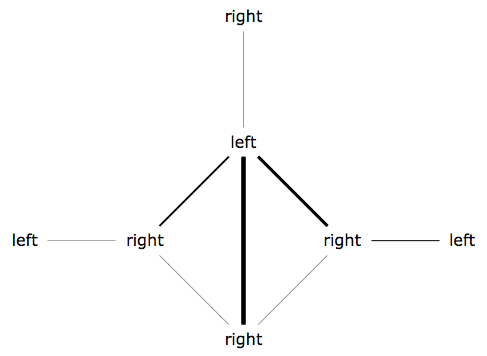
\includegraphics[width=8cm, height=6cm]{taking-sides-graph.png}\\
%  \caption{Grafo extraído de \cite{malouf-taking_sides}. Os vértices são usuários e as arestas, citações entre eles. Arestas mais escuras indicam frequência de citação mais alta.}
%  \label{fig:malouf}
%\end{figure}


%Padrões de citação a \emph{sites} também foram investigados \cite{efron}. No artigo de Miles Efron, os experimentos envolvem os \emph{datasets} \textbf{Political-Orientation} e \textbf{Artists}. O primeiro é composto de artigos políticos Estadunidenses de Direita ou Esquerda e o segundo é composto de textos sobre artistas musicais, divididos entre as categorias Alternativo e Popular. As taxas de acerto relatadas para as aplicações de Naïve Bayes nestes corpora foram de, respectivamente, 64.71\% e 50.1\%. A fim de melhorar as taxas de acerto na classificação dos documentos, o artigo estima a perspectiva de cada um deles avaliando a probabilidade de que eles sejam co-citados, na Web, com documentos referência de cada perspectiva. Estes documentos de referência são agrupados em listas de URLs. Esta metodologia, aplicada a \textbf{Political-Orientation}, resultou em uma taxa de acerto de 94.1\%. Para \textbf{Artists}, a taxa de acerto máxima obtida foi de 88.84\%.

%Todos os artigos que propuseram metodologias para melhorar a classificação em corpora com vocabulários muito uniformes consideraram algum esquema de citação. Se o corpus for composto de documentos pouco citados na Web, o esquema do artigo de Miles Efron pode não trazer nenhuma melhoria significativa ao problema. Se os autores dos documentos não mencionarem significativamente um ao outro, como aconteceu nos estudos com o \emph{dataset} \textbf{Politics}, a metodologia explorada por Tony Mullen e Robert Malouf não é recomendada. Essa área de pesquisa, portanto, ainda tem alguns problemas em aberto - e, considerando que estes três artigos foram escritos há mais de quatro anos, ela não parece atrair muita atenção. A justificativa para isso, provavelmente, tem a ver com o fato de que uniformidade no vocabulário não é um problema tão comum em Mineração de Perspectiva. No \textbf{capítulo X}, técnicas envolvendo comparação entre documentos, que podem trazer benefícios à classificação de \emph{datasets} difíceis - e neste caso também se enquadram aqueles em que o vocabulário é mais uniforme -, serão discutidas.

\section{Conclusões}
\label{freqs:conc}

%INTERNACIONALIZÁVEEEEEL!!

%classif. com contagens rocks, l-lda rocks, qto mais diferente melhor, mas pelos resultados obtidos na revisão, parece q eh bem por aí.

A classificação baseada em contagens de palavras, ou em alguma das variações mencionadas na introdução desse capítulo, assume a seguinte hipótese linguística: a quantidade de vezes que uma palavra é mencionada em um documento está diretamente relacionada a seu enfoque \cite{teubert}. Como consequência, esse método funciona melhor em \emph{datasets} nos quais o emprego de palavras varia significativamente por perspectiva. Esse parece ser o caso da maioria dos artigos estudados para este capítulo: cinco de seis trabalhos apresentaram uma boa taxa de acerto, considerando apenas contagens de palavras. Outros três trabalhos, apresentados no capítulo \ref{outros}, também fazem uso dessa informação - mas a associam a outras propriedades dos documentos classificados. De todo modo, a contagem de palavras mostrou ser a característica mais \textbf{essencial} à classificação por perspectiva, reforçando a ideia de que essa hipótese linguística é válida.


Nesse capítulo, foram revisados dois trabalhos que utilizam apenas essas contagens para classificar seus \emph{datasets} de estudo - eles são, inclusive, os mais citados dentre os treze analisados nessa monografia.

O primeiro, de Lin et al., apresenta um novo modelo para classificação (o LSPM), destacando-se dos demais artigos por não enfocar em SVMs ou Naïve Bayes. Diferentemente desses classificadores, o LSPM considera que apenas uma parte das sentenças de cada documento realmente apresenta um ponto de vista, e gera palavras mais específicas para cada uma delas. As demais frases concentram palavras mais genéricas, que poderiam ser empregadas da mesma forma por todos os lados do corpus. Por esse motivo, elas não contribuem diretamente com a classificação. O modelo apresenta uma boa taxa de acerto, mas não é tão estudado - nem tão trivial de implementar - quanto um Naïve Bayes. O trabalho é muito citado por ser um dos primeiros a tentar classificar documentos de acordo com suas perspectivas, e o \emph{dataset} analisado (artigos pró-Israel e pró-Palestina) também foi estudado por outros pesquisadores\footnote{Verificar \textbf{ANEXO BLA}.}.

O segundo, de Mullen e Malouf, é muito citado por ser um dos poucos que trabalha com um \emph{dataset} tão informal (\emph{posts} em um fórum sobre política), apresentando discussões interessantes sobre as dificuldades envolvidas no processo de classificá-lo. As taxas de acerto obtidas na classificação foram baixas, e um dos motivos possíveis, de acordo com o exposto no trabalho, é a quantidade de citações a textos escritos sob uma perspectiva diferente daquela que o autor defende. Isso \emph{mistura} contagens relativas a perspectivas distintas em um mesmo documento, homogeneizando-os sob o ponto de vista do classificador. 

O artigo de Lin et al. também apresentou uma boa taxa de acerto utilizando um Naïve Bayes, diferentemente do estudo de Mullen e Malouf. Apesar do corpus analisado por esses últimos ser pequeno, os autores indicam que a forma como cada perspectiva se apropria das palavras interfere na qualidade da classificação.  A fim de ampliar a compreensão sobre essa interferência, foram conduzidos dois experimentos envolvendo um Naïve Bayes e um L-LDA, aplicados a \emph{datasets} para os quais a classificação funcionou de forma diferente. O primeiro corpus considerado foi aquele estudado por Lin et Al., para o qual as taxas de acerto obtidas com um Naïve Bayes foram altas; o segundo, dado que não foi possível ter acesso aos documentos analisados por Mullen e Malouf, foi um conjunto de trechos de discursos em debates da \emph{House of Representatives}, órgão legislativo dos Estados Unidos. A taxa de acerto obtida com um Naïve Bayes nesse último corpus foi bastante baixa, tornando-o ideal para o objetivo dos experimentos. 

Nos experimentos com o L-LDA, cada documento foi associado a dois tópicos: um genérico e outro correspondente à sua perspectiva. Mesmo sabendo que em um Naïve Bayes não há distinção entre palavras genéricas e específicas, optou-se por essa divisão de tópicos por conta do objetivo da aplicação do L-LDA: a visualização parcial de que termos são mais enfocados por cada perspectiva. Essa informação sugere que há uma certa homogeneização nos enfoques do segundo \emph{dataset}, quando comparado com o primeiro. Considerando que quão mais homogêneo é o emprego de palavras por perspectiva, pior é o desempenho dos classificadores baseados em contagens de palavras, a informação obtida com o L-LDA ajuda a compreender porque a taxa de acerto obtida para o segundo \emph{dataset} foi tão mais baixa que aquelas obtidas para o primeiro. É importante frisar que não se encontrou \textbf{nenhum outro trabalho} que faça uso de um L-LDA para compreender, ainda que parcialmente, como certos termos são enfocados por diferentes perspectivas. Apesar de outros fatores contribuírem para o mau desempenho de uma classificação, como um número muito pequeno de documentos no \emph{dataset}, a investigação do emprego de palavras, quando as taxas de acerto obtidas não são boas, amplia a compreensão do corpus analisado - o que pode ser útil no momento de se pensar em outras estratégias para melhorar a classificação.  

%é interessante, para um classificador baseado em contagens de palavras, que elas variem o quanto for possível de uma perspectiva para outra, evidenciando os diferentes enfoques e pontos de vista dos autores dos documentos, a informação obtida com o L-LDA explica, ainda que  
 %, para compreender melhor como os autores dos documentos se expressam. % Se as palavras são empregadas de modo muito parecido por todas as perspectivas, isto justifica, ainda que em parte, o mau desempenho obtido. 

% Considerando que a classificação dos dois \emph{datasets} baseou-se apenas em contagem de palavras, a informação obtida com o L-LDA ampliou a discussão %m isso, e considerando a taxa de acerto obtida com o Naïve Bayes em cada caso,  % facilitou a visualização sobre aquilo que é mais específico de cada perspectiva. Como o uso do L-LDA objetivava apenas a uma 

%de modo que % A ideia era ilustrar, através de um L-LDA, o emprego de palavras em um corpus bem classificado com %e foi por este motivo que esse %a relevância das contagens de palavras para classificação por perspectiva é patente% De acordo com a revisão, cinco doos seis artigos , cinco apresentaram um bom 

%Este capítulo apresentou duas hipóteses linguísticas assumidas por métodos baseados em frequências de palavras: 1) palavras específicas, denominadas \emph{banner words}, costumam ser utilizadas para defender perspectivas diferentes e 2)   %tão melhor quanto mais diferentes forem os empregos de palavras por perspectiva.

%ideia de que pessoas costumam utilizar palavras específicas, denominadas \emph{stigma words} ou \emph{banner words}, para defender perspectivas diferentes. O uso de classificadores baseados na presença ou frequência das palavras, portanto, costuma funcionar bem na identificação dessas perspectivas. Entretanto, em alguns casos, as construções do discurso refletem diferentes perspectivas melhor do que o uso de palavras específicas. Nestes casos, as taxas de acerto desses classificadores são menores do que o desejado. 

%Para ilustrar a relação entre as palavras de dois \emph{datasets} e o desempenho desses métodos, experimentos com o modelo de tópicos L-LDA foram executados. A extração das dez palavras mais fortemente associadas a cada tópico conduziu à visualização parcial de como o vocabulário dos \emph{datasets} se agrupa em torno de suas diferentes perspectivas. A informação, apesar de subjetiva, auxilia na compreensão das taxas de acerto obtidas com um classificador Naïve Bayes padrão, aplicado aos dois corpora. Para o primeiro \emph{dataset}, as taxas de acerto obtidas foram mais altas, o que pode ser explicado por uma presença maior de \emph{banner words} em comparação com o segundo \emph{dataset}.



% voa relação entre as palavras contidas em dois \emph{datasets} e suas diferentes perspectivas. No primeiro \emph{dataset}, as palavras extraídas para cada perspectiva se relacionam, semanticamente, melhor com a perspectiva em si do que no segundo \emph{dataset}. Neste último, palavras genéricas, como artigos e conjunções, se associam muito fortemente a todas as perspectivas, colaborando para uma uniformização do vocabulário. Isto explica, ainda que não seja trivial avaliar o quanto, as taxas de acerto mais altas obtidas com um Naïve Bayes no primeiro \emph{dataset}.

%Por fim, este capítulo também revisa artigos que discutem a questão do vocabulário do corpus. Estes artigos propõem metodologias para melhorar a classificação em \emph{datasets} cujo vocabulário é considerado muito uniforme - todas baseadas em algum esquema de citação a documentos. A questão do vocabulário do corpus é pouco discutida na literatura; provavelmente porque o problema é pouco comum e porque outros métodos, mais genéricos para \emph{datasets} difíceis de classificar, têm sido mais estudados.
 
%o primeiro \emph{dataset}, os artigos estão escritos sob uma das seguintes perspectivas: pró-Palestina ou pró-Israel. Por conta disso, o tópico \emph{pal} foi atribuído a todos os documentos pró-Palestina e o tópico \emph{isr}, a todos os pró-Israel. Estes tópicos facilitam a visualização das palavras mais fortemente associadas a cada uma das duas perspectivas, de acordo com o vocabulário empregado nos artigos. Um terceiro tópico, \emph{gen}, foi atribuído a todos os documentos, a fim de capturar as palavras que co-ocorrem neles independentemente de suas perspectivas. Após a execução do modelo, as 100 palavras mais fortemente associadas a cada um dos 3 tópicos foram coletadas. 35\% das associadas a \emph{isr} não estão presentes no conjunto recolhido para \emph{gen}. Para \emph{pal}, essa percentagem cai para 29\%. Por fim, 32\% das palavras mais fortemente associadas a \emph{isr} não fazem parte das 100 palavras mais fortemente associadas a \emph{pal} e vice-versa. Essas percentagens indicam que os autores dos documentos pró-Israel utilizam um vocabulário ligeiramente mais específico, na defesa de seus pontos de vista, do que os autores pró-Palestina. É importante ressaltar que nenhuma palavra foi filtrada na análise - ou seja, termos muito frequentes como \emph{the}, \emph{of} e \emph{and}, comumente extraídos dos \emph{datasets} antes da etapa de classificação, estavam presentes nos documentos processados pelo L-LDA.    

%Palavras associadas a \emph{isr} que não foram associadas a \emph{gen}
%['arafat', 'be', 'some', 'roadmap', 'us', 'yet', 'out', 'sharon', 'ariel', 'support', 'three', 'bush', 'palestine', 'new', 'terrorism', 'leader', 'then', 'jewish', 'after', 'arab', 'leadership', 'plan', 'president', 'than', 'bank', 'prime', 'regarding', 'like', 'could', 'violence', 'against', 'while', 'time', 'american', 'first']

%Palavras associadas a \emph{pal} que não foram associadas a \emph{gen}
%['then', 'some', 'authority', 'against', 'occupied', 'negotiations', 'occupation', 'sharon', 'united', 'end', 'way', 'palestine', 'international', 'be', 'after', 'plan', 'president', 'law', 'those', 'prime', 'land', 'i', 'violence', 'us', 'q', 'while', 'time', 'situation', 'first']

%Palavras associadas a \emph{pal} que não foram associadas a \emph{isr}
%['because', 'people', 'authority', 'states', 'right', 'occupied', 'any', 'negotiations', 'occupation', 'what', 'united', 'end', 'also', 'been', 'their', 'other', 'way', 'international', 'law', 'do', 'which', 'government', 'very', 'they', 'now', 'those', 'about', 'land', 'these', 'q', 'i', 'situation']

%Palavras associadas a \emph{isr} que não foram associadas a \emph{pal}
%['arafat', 'into', 'settlements', 'years', 'yet', 'out', 'even', 'would', 'ariel', 'west', 'support', 'three', 'bush', 'gaza', 'new', 'terrorism', 'leader', 'we', 'jewish', 'arab', 'most', 'leadership', 'minister', 'roadmap', 'than', 'bank', 'both', 'regarding', 'like', 'could', 'war', 'american']
%\textbf{As palavras estão ordenadas de acordo com a força da associação com cada um dos tópicos}


%\textbf{Lista de palavras e desempenho. Imagens e Tabelas.}

%Dado que em boa parte dos artigos estudados neste projeto, como \cite{lin-et-al2006} e \cite{klebanov}, atinge-se taxas de acerto superiores a 80\% com classificadores baseados em frequência de palavras, conclui-se que a mineração de perspectivas em discussões, artigos opinativos e debates requer metodologias diferentes, a depender de como as palavras foram escolhidas pelos autores dos documentos. %Nos debates estudados por \cite{hirst-et-al}, expressões de ataque e defesa são mais frequentes do que \emph{stigma words} e, como o método empregado no artigo foi um SVM treinado com frequências de palavras, observou-se que a classificação obtida para os lados do debate não refletia as perspectivas \emph{liberal} ou \emph{conservadora} - mas sim os lados \emph{oposição} (expressões de ataque) e \emph{situação} (expressões de defesa). 
%Estes estudos indicam a possibilidade de que, em debates e discussões nos quais há uma homogeneização do vocabulário empregado - o que pode acontecer quando todos os lados utilizam, em proporções similares, tanto expressões de ataque quanto de defesa -, classificadores baseados exclusivamente nas palavras utilizadas e/ou em suas frequências apresentarão má performance.

%A avaliação do desempenho desses classificadores\footnote{\textbf{SVMs e Naive Bayes padrão; LSPM}} nos \emph{datasets} estudados revela que artigos opinativos e notícias consolidaram perspectivas, através da escolha do vocabulário utilizado, melhor do que debates. Apesar disso, uma generalização neste sentido, restringindo o uso desses classificadores a artigos e notícias, não é recomendada por falta de indicativos linguísticos que comprovem essa tendência. Uma estratégia que pode ajudar na escolha ou descarte de um classificador desse tipo é uma análise das palavras que estão contidas nos documentos.

%\textbf{mostrar as percentagens prum dataset onde a linguagem eh mais uniforme. discutir.} 
%Explicar q isso nunca foi feito e q pessoas q ncontraram merda com essa feature fizeram outras coisas. descrever essas coisas.

%Estas hipóteses ilustram  
%Como indica \cite{}: 

%\textbf{MODO RASCUNHO AINDA}

%Explicar que uma diferença fundamental notada entre os datasets observados diz respeito à formalidade da linguagem empregada nos documentos. Enquanto alguns datasets utilizam documentos provenientes de meios onde a norma culta da linguagem impera, e uma revisão ortográfica é utilizada, outros são carregados de gírias, expressões e abreviações típicas da linguagem da Internet e contêm, eventualmente, grafias erradas para uma mesma palavra. <Dar exemplos textuais. Mostrar uma tabelinha, algo assim, indicando o volume de datasets com linguagem informal nos documentos estudados.> 

%A linguagem informal pode criar alguns desafios para a Mineração de Perspectiva [FECHAR O PROBLEMA EM: IDENTIFICAÇÃO DA PERSPECTIVA PRESENTE EM UM DOCUMENTO], especificamente no que diz respeito ao pré-processamento dos documentos e à escolha do método empregado. No pré-processamento, como indicado em (aaai-politics.pdf e 10.1.1.138.7160.pdf), a correção gramatical das palavras é bastante indicada. Com uma única versão de grafia para cada palavra (a correta), diminui-se a quantidade de ruído que grafias erradas podem causar na classificação.

%Uma característica dos datasets que deveria ser considerada sempre antes de se escolher o método utilizado - mas não é prática entre as pessoas que estudam perspective mining - é a frequência das palavras nos documentos do dataset. Se o léxico empregado pelos autores dos textos muda sensivelmente a depender de sua ideologia/perspectiva defendida/ponto de vista, é possível resolver o problema utilizando classificadores que usam essa frequencia como feature. GASTE TEMPO DANDO ALGUNS EXEMPLOS.  Em datasets informais, entretanto, como aponta Efron, a linguagem empregada por todos os lados da discussão pode ser basicamente a mesma: termos com forte carga de polaridade e gírias/jargões comuns na discussão [EXEMPLO]. Neste caso, é preciso utilizar métodos que utilizem mecanismos mais rebuscados do que a simples frequência/presença das palavras no texto. Alguns autores utilizam métodos mais gramaticais para lidar com datasets informais, como é o caso de , BLE e BLI. Os 2 primeiros criam o conceito de Opinion Frame (DEFINIR O CONCEITO). No primeiro caso, a ideia é associar corretamente opiniões a alvos, e associar alvos iguais utilizando técnicas de co-referência. Segundo Wiebe et al. (pegar a citação corretamente), ter as targets associadas, com as opiniões próximas, é uma boa forma de entender o overall de opiniões de um documento. A estratégia é uma alternativa possível para documentos em que as perspectivas estão muito associadas à linguagem opinativa, e onde essa linguagem é comum para todos os lados. Infelizmente, os resultados alcançados indicam que a tarefa não é trivial: blablablablababla (resolver coreferencia pra linkar targets não é tão simples assim => e dê exemplo). 

%uma diferença fundamental notada entre os \emph{datasets} observados diz respeito à formalidade da linguagem empregada nos documentos. Enquanto alguns datasets utilizam documentos provenientes de meios onde a norma culta da linguagem impera, e uma revisão ortográfica é utilizada, outros são carregados de gírias, expressões e abreviações típicas da linguagem da Internet e contêm, eventualmente, grafias erradas para uma mesma palavra. <Dar exemplos textuais. Mostrar uma tabelinha, algo assim, indicando o volume de datasets com linguagem informal nos documentos estudados.> 

%\begin{table}[t]
%\centering
%\begin{tabular}{| p{10cm} | }
%\hline

%\emph{"The recent \textbf{Israeli} government decision to begin building extensive walls
%around \textbf{Palestinian} is just one more example of how \textbf{Israeli} Prime
%Minister Ariel Sharon is unable to deal with \textbf{Israeli} problems save
%through his narrow security vision."} - Trecho extraído de artigo Pró-Palestina. \\ \hline

%\emph{"The first conclusion that the Israeli political and security
%establishment should learn and internalize after 18 months of
%\textbf{Palestinian} Intifada, concerns the intensity of \textbf{Palestinian} blind
%terrorism and guerilla warfare against the State of Israel."} - Trecho extraído de artigo Pró-Israel. \\ \hline

%\end{tabular}
%\label{3}
%\caption{Trechos com as palavras \emph{palestinian} e \emph{israeli}, extraídos do \emph{dataset} \textbf{Bitterlemons}.}
%\end{table}

%\begin{table}[t]
%\centering
%\begin{tabular}{| p{10cm} | }
%\hline

%\emph{"\textbf{Bush}
%and his advisers, who have been critical of Clinton's deep involvement
%in a failed peace process ever since taking office, nevertheless
%understood at the time that peace in the Middle East should be beyond
%politics in America, and that the US could not permit itself to turn its
%back on an Israeli leader who was determined to make peace."} - Trecho extraído de artigo Pró-Israel. \\ \hline

%\end{tabular}
%\label{4}
%\caption{Trecho com a palavra \emph{bush}, extraído do \emph{dataset} \textbf{Bitterlemons}.}
%\end{table}

%\begin{table}[t]
%\centering
%\begin{tabular}{| p{10cm} | }
%\hline
%\emph{"But just as we were close to a complete
%package that would have ended the \textbf{occupation} and established a
%Palestinian state, Barak permitted Ariel Sharon's provocative visit to
%Al Aqsa mosque, and launched his "revenge" on Palestinians."} - Trecho extraído de artigo Pró-Palestina. \\ \hline
%\end{tabular}
%\label{5}
%\caption{Trecho com a palavra \emph{occupation}, extraído do \emph{dataset} \textbf{Bitterlemons}.}
%\end{table}
% e  Termos associados ao Governo dos Estados Unidos, como \emph{bush} e \emph{american}, ilustram a relevância da aliança política estabelecida por Israel à época dos documentos. Palavras como \emph{occupation} e \emph{people}, por outro lado, ilustram a principal pauta Palestina no mesmo período: a ocupação da Faixa de Gaza.

%Os artigos deste primeiro \emph{dataset} foram escritos ou pelos editores do \emph{site} ou por convidados, divisão utilizada em \cite{lin-et-al2006} para avaliar o desempenho de um Naïve Bayes. No primeiro cenário, os documentos de treinamento eram os escritos pelos editores e os de teste, aqueles escritos pelos convidados; no segundo, tinha-se a situação inversa.

%As taxas de acerto obtidas com um classificador Naïve Bayes na identificação das perspectivas pró-Israel e pró-Palestina variaram entre 73.47\% e 98.98\%, a depender da divisão entre os conjuntos de treinamento e teste. %disponível em \cite{alibezz-nb}, as taxas de acerto obtidas foram de 73.47\% e 98.98\% para cada um dos cenários, respectivamente\footnote{A taxa de acerto obtida para o primeiro cenário foi significativamente inferior à obtida em \cite{lin-et-al2006} (85.85\%). Provavelmente, isto tem a ver com o número de iterações e as condições iniciais da execução.}. 

%O segundo \emph{dataset} estudado é o \textbf{Convote-Menor}, composto de colocações em debates da \emph{House of Representatives}, um dos dois órgãos principais do poder legislativo federal dos Estados Unidos. Os documentos foram marcados como sendo de parlamentares Republicanos ou Democratas, e como representando um posicionamento a favor ou contra a lei em pauta. Para este experimento, apenas a divisão entre Republicanos e Democratas foi considerada. O L-LDA foi aplicado a este \emph{dataset} de forma análoga ao primeiro experimento, e as dez palavras mais fortemente associadas a cada um dos tópicos - Genérico, Republicano e Democrata - estão listadas na Tabela 4.2. \emph{Stop words} também foram excluídas desta listagem.

%Ele é parte de um \emph{dataset} maior estudado pela primeira vez em \cite{thomas-pang-lee}, e está disponível em \cite{alibezz-convote}. A rotulação original dos documentos foi mantida neste \emph{dataset}: cada um deles é marcado com R, caso represente a colocação de um Republicano; ou D, no caso Democrata. Os documentos também são marcados com Y, caso representem a colocação de alguém que votou pela aprovação de uma lei; ou N, em caso contrário. Esta segunda marcação não foi explorada nesta monografia, nem a combinação das duas. O que se analisou, portanto, foi o desempenho do Naïve Bayes, disponível em \cite{alibezz-nb}, na classificação dos documentos como Republicanos ou Democratas.

%O L-LDA foi aplicado a este \emph{dataset} de forma análoga ao primeiro experimento, aproveitando os rótulos R e D, presentes nos documentos, como tópicos, e utilizando também um tópico genérico. As trinta palavras mais fortemente associadas a cada um dos tópicos, em ordem, podem ser conferidas na Tabela abaixo:

